\begin{savequote}
It is precisely this variation -- and the apparent success of our visual system
and brain in achieving recognition in the face of it -- that makes the problem
of pattern recognition so interesting.
\qauthor{Irving Biederman, \textit{Higher-level vision}}
\end{savequote}
\chapter{Hand Features and Representations}
This chapter discusses different 
hand feature representations and encoding methods to produce feature
vectors as input to the recognition module.  One feature vector is computed
for each input frame streamed from the sensor(s) to form a sequence of feature
vectors.

As features can have different numeric ranges, to avoid features with greater
numeric ranges dominating those with smaller numeric ranges, it is important to
scale the feature vectors before feeding them  into the recognition
module~\cite{hsu10}. Hence, after computing the feature vectors, the last step
is always standardizing all the features to have 0 mean and 1 standard deviation
using all the training data. During testing, the data are standardized using the means and the standard deviations from training.

\section{Hand Motion Features}
Motion features are important for path gesture representation. 

It is relatively easy to obtain motion features from IMUs if they are present.
From the ChAirGest dataset, I use linear acceleration $(x, y, z)$,
angular velocity $(x, y, z)$ and Euler orientation (yaw, pitch, roll) from the
IMU on the hand to form a 9-dimensional feature vector
$\underline{x}_t^{\text{imu}}$ at every time frame $t$.

One limitation of IMUs is that they cannot provide hand position information. To
complement this, we can use hand position information from hand tracking in the
previous section. With the Kinect sensor data from the ChAirGest dataset and
using the gesture salience based hand tracking method, I extract the position of a gesturing hand in $(x, y, z)$ coordinates relative to the shoulder center joint to form a 3-dimensional vector $\underline{x}^\text{kinect}_t$ (should center joint position from the Kinect
SDK is relatively accurate under most situations).
Combining the two, we
have a 12-dimensional feature vector $\underline{x}_t =
[\underline{x}^\text{kinect}_t, \underline{x}^\text{imu}_t]$.
The evaluation in Table~\ref{tab:comp-motion-feature} shows that adding
position information can improve recognition accuracy further for path gestures. 

\begin{table}[tbh]
\begin{center}
\begin{tabular}{|l|p{6cm}|p{4cm}|}
\hline
 & Hand position from salience detection \& IMU,
 $[\underline{x}^\text{kinect}_t, \underline{x}^\text{imu}_t]$ & IMU only, $\underline{x}^\text{imu}_t$ \\
\hline
F1 Score & \textbf{0.907 (0.01)} & 0.890 (0.02) \\
\hline
ATSR Score & \textbf{0.923 (0.02)}  & 0.920 (0.01) \\
\hline
Final Score & \textbf{0.912 (0.01)}  & 0.895 (0.01) \\
\hline
\end{tabular}
\caption{Comparison of the average 3-fold cross validation results for different
motion feature vectors. Values in parentheses are standard deviations.}
\label{tab:comp-motion-feature}
\end{center}
\end{table}

If no IMU is present, we can still compute velocity and acceleration from
relative positions.
It is useful to apply temporal smoothing on the motion data. In the
real-time system, I apply ``box'' smoothing (i.e., simple linear smoothing
with equal weights) with a window size of 15 frames on the relative positions of
the gesturing hand.

Figure~\ref{fig:motion-hist-rest} shows the histograms of the standardized $(x,
y, z)$ coordinates of relative position, velocity and acceleration from one user's
data in the YANG dataset. The peak values corresponds to the rest position
because it is the most frequent pose in the recording.
Figure~\ref{fig:motion-hist} shows the histogram of the same data excluding
those from the rest position. We can see that the distribution roughly follows
Gaussian or mixture of Gaussians distributions.

\begin{figure}[!tbh]
\centering
\subfigure[With rest positions.]{
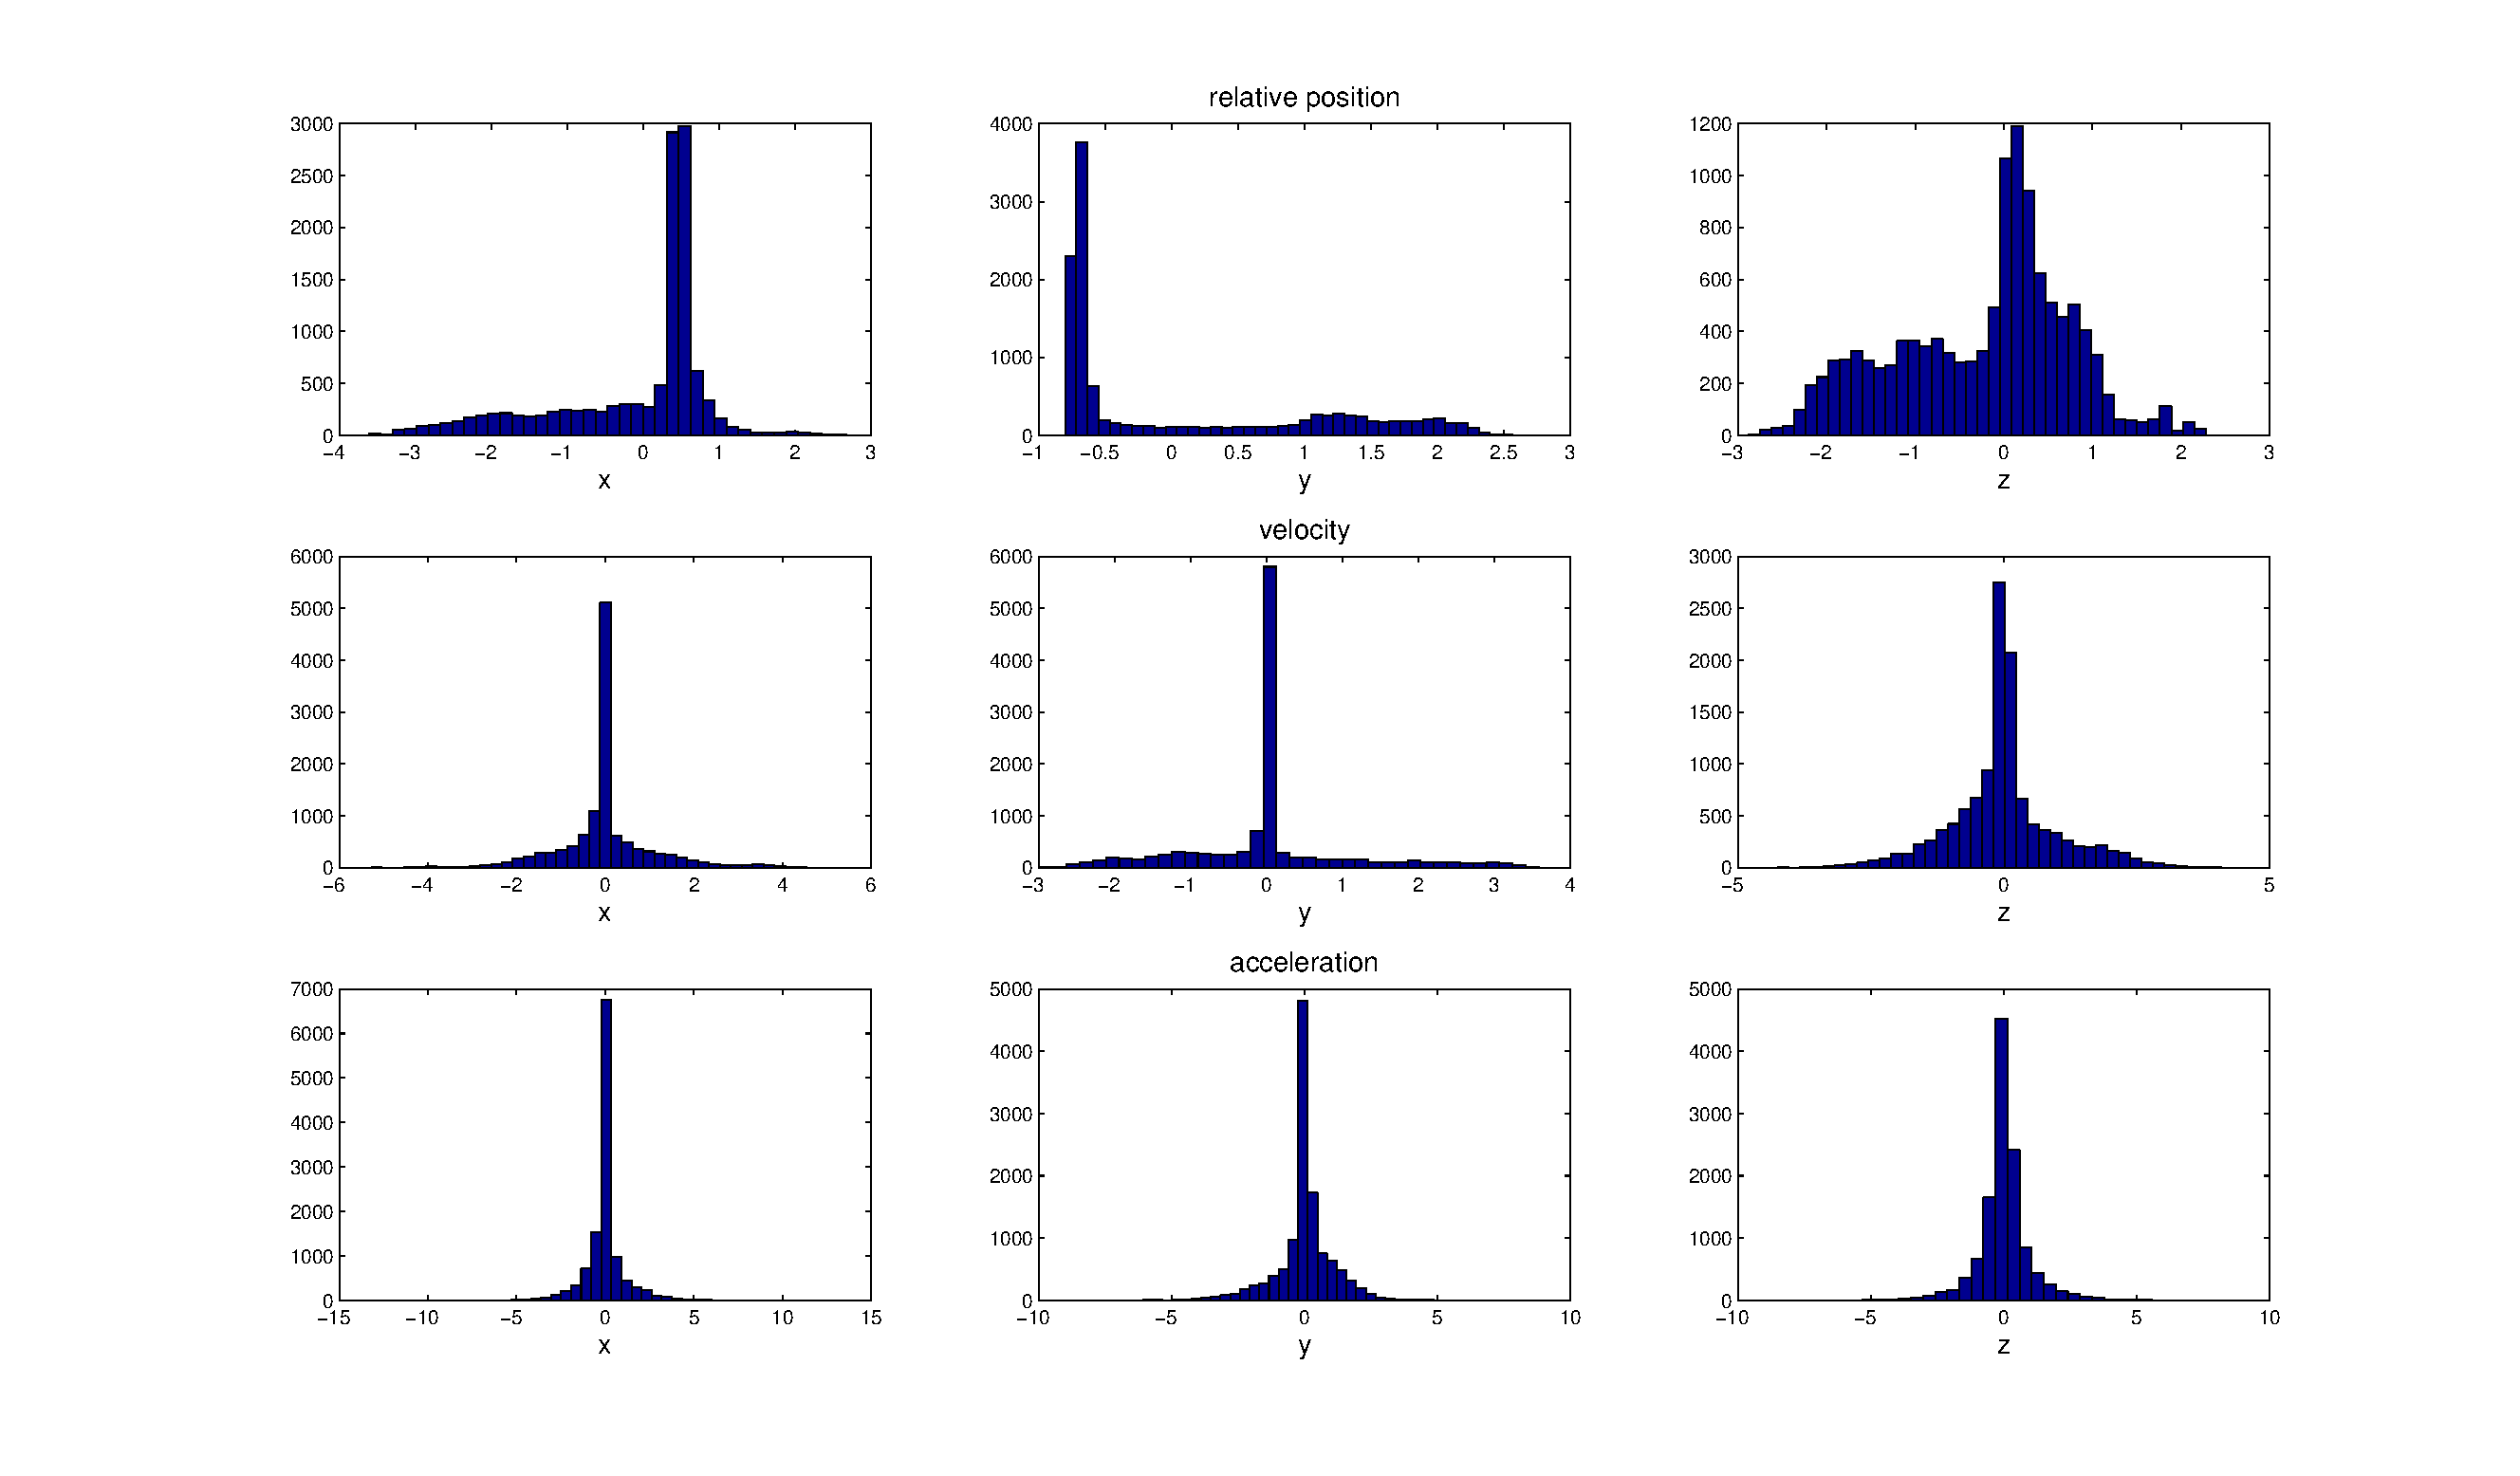
\includegraphics[trim=30mm 15mm 30mm 10mm,
clip, width=0.97\columnwidth]{figures/motion_hist_rest.eps}
\label{fig:motion-hist-rest}
}
\subfigure[Without rest positions.]{
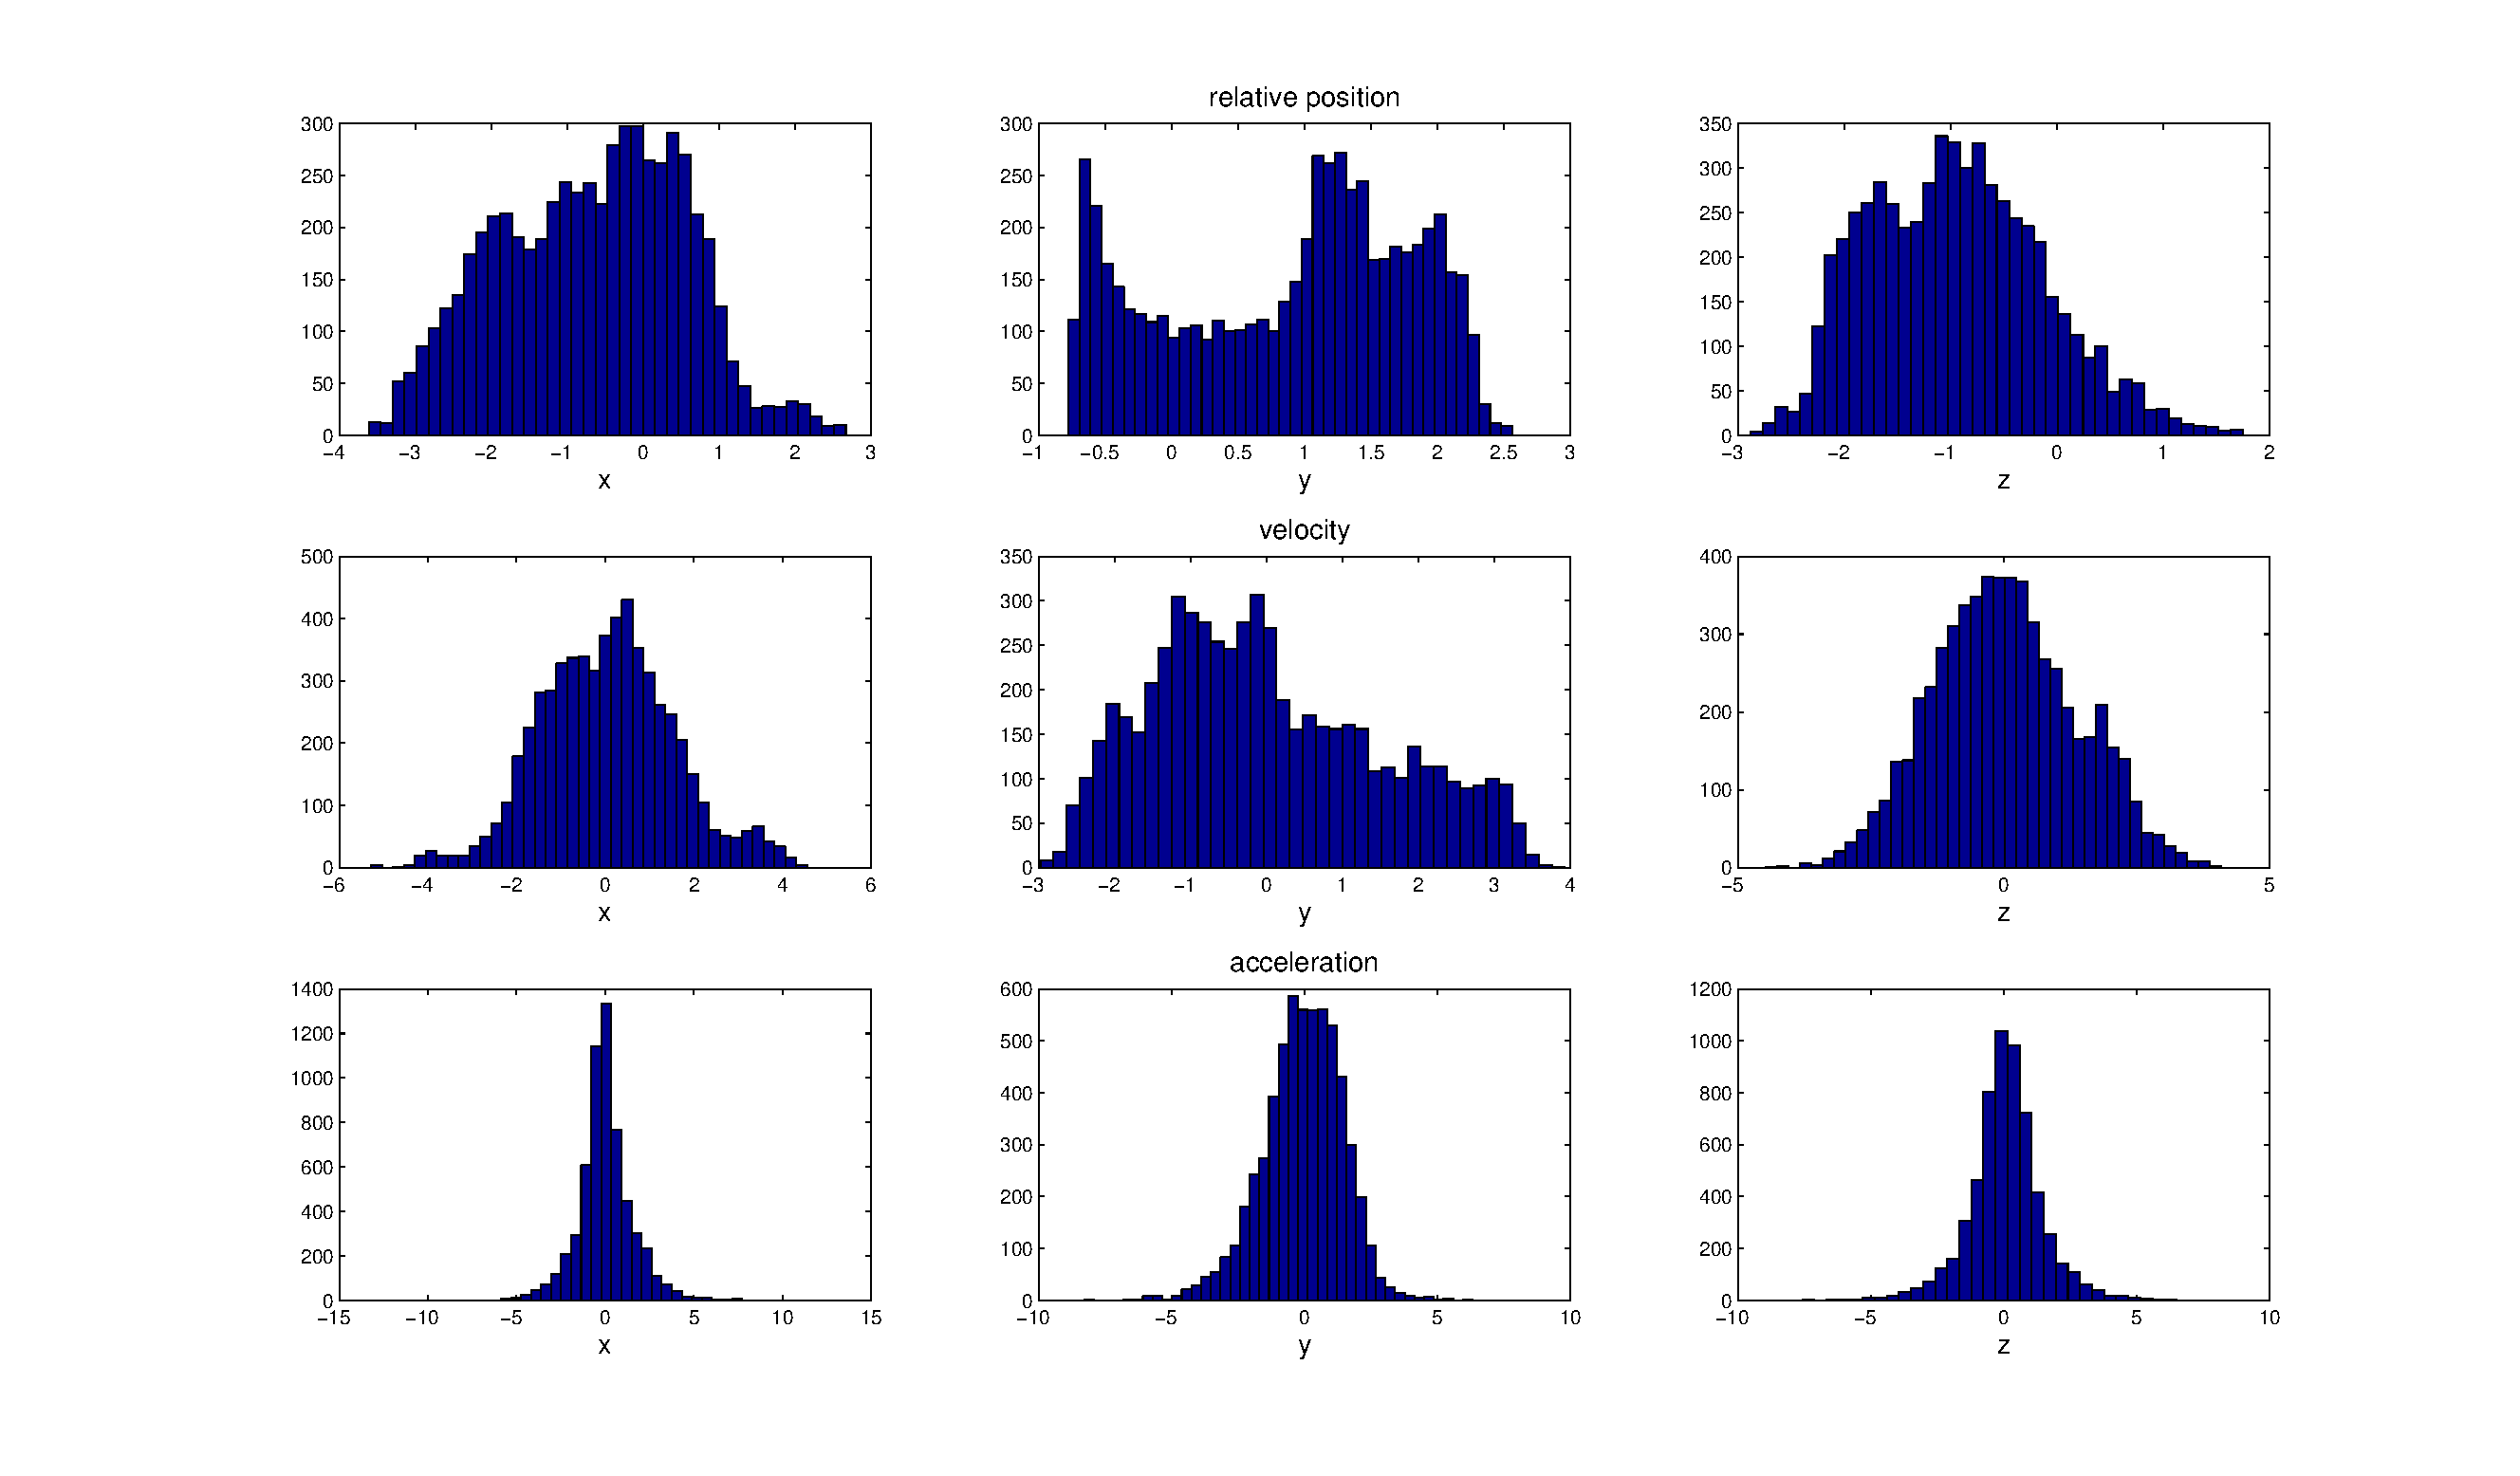
\includegraphics[trim=30mm 15mm 30mm 10mm,
clip, width=0.97\columnwidth]{figures/motion_hist.eps}
\label{fig:motion-hist}
}
\caption{Histograms of motion features.}
\end{figure}

%Try Xsens data on hand, quarternion.

\section{Hand Pose Features}
I use HOG as the feature descriptor for hand poses. The HOG feature descriptor
can be computed from either color, depth or both images. Figure~\ref{fig:hand}
shows sequences of hand image patches extracted using the salience based hand
tracking algorithm. The depth gray images are obtained by scaling the depth
values between 0 -- 255.

\begin{figure}[tbh]
  \centering
  \subfigure[Gray images converted from color images with only skin-colored
  pixels.] {
	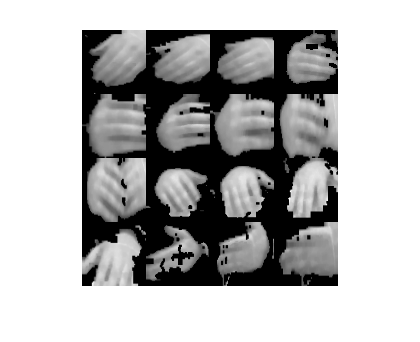
\includegraphics[width=0.45\textwidth]{figures/color_hand.png} 
  }
  \subfigure[Corresponding depth-mapped images.] {
  	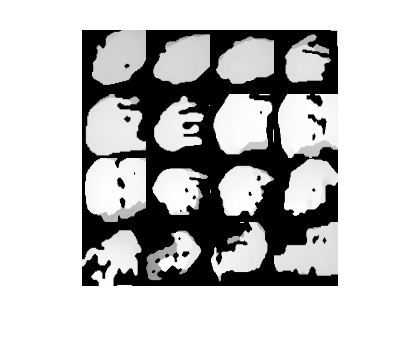
\includegraphics[width=0.45\textwidth]{figures/depth_hand.png}
  }
  \caption{$64\times64$px raw image patches of hands from the ChAirGest
  dataset.}
  \label{fig:hand}
\end{figure}

\subsection{Histogram of Oriented Gradients (HOG)}
For each pixel, the magnitude ($r$) and the orientation ($\theta$) of the
gradient are
\begin{align*}
r &= \sqrt{dx^2 + dy^2} \\
\theta &= \text{arccos}(dx / r) 
\end{align*}
where $dx$ and $dy$ are computed using a centered $[-1, 0, 1]$ derivative mask.
Each pixel contributes a weighted vote (the magnitude of the gradient $r$) to an
edge orientation histogram based on the orientation, $\theta$, of the gradient
element centered on it, and the votes are accumulated into orientation bins over local spatial regions called
\textit{cells}.
The orientation bins are evenly spaced over 0\textdegree -- 180\textdegree
(``unsigned'' gradient). To reduce aliasing, votes are interpolated
bilinearly between the neighboring bin centers in both orientation and
position~\cite{dalal05}. 

Fine orientation and spatial binning turns out to be essential for good
performance. My evaluation shows that using $4\times 4$px cells
(\texttt{cell\_size} = 4) and 9 orientation bins gives the best result.

Finally, cell values are normalized using blocks of $2\times 2$ cells
(Figure~\ref{fig:cell}).
If an image $I$ has dimensions $m\times n$, the size of the computed feature vector
$H$ is $(m/\texttt{cell\_size} - 1) \times (n/\texttt{cell\_size} - 1) \times
\texttt{num\_bin}$. Figure~\ref{fig:hand-hog} hows a visualization of the HOG
descriptors from both the color images and depth-mapped images.

\begin{figure}[!tbh]
\centering
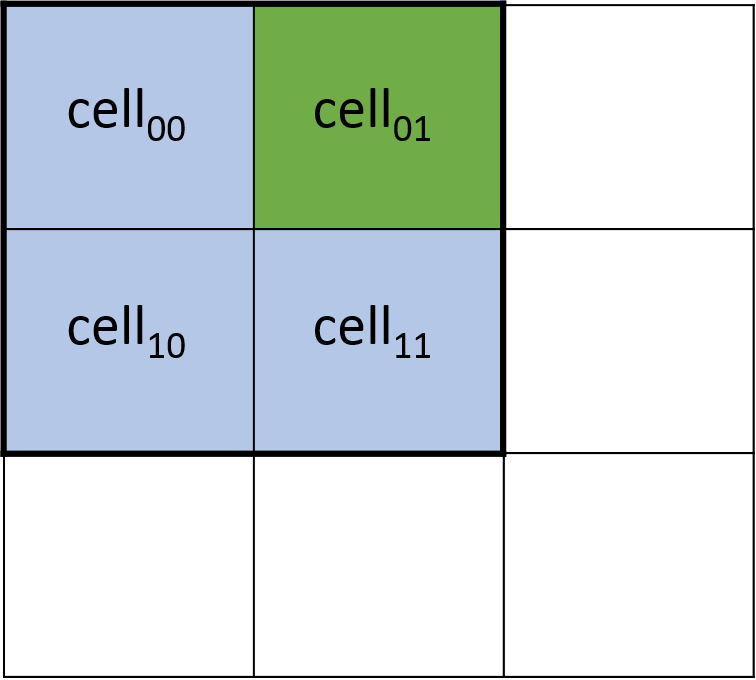
\includegraphics[width=0.3\textwidth]{figures/cell.png}
\caption{Histogram values in $\text{cell}_{01}$ is normalized by the sum in
$\text{cell}_{00}$, $\text{cell}_{01}$, $\text{cell}_{10}$,
and $\text{cell}_{11}$.
}
\label{fig:cell}
\end{figure}

\begin{figure}[!tbh]
  \centering
  \subfigure[Gray images converted from color images.] {
  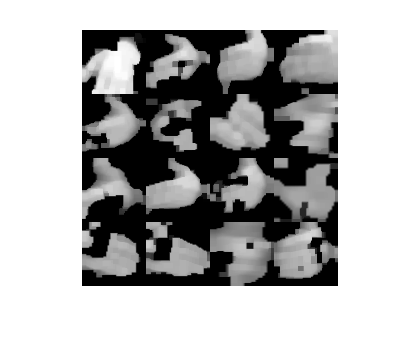
\includegraphics[trim=10mm 15mm 10mm 5mm,
clip,width=0.45\textwidth]{figures/color_denoised_5.png} 
  }
  \subfigure[Corresponding depth-mapped images.] {
    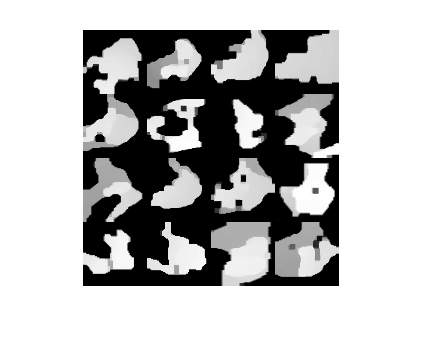
\includegraphics[trim=10mm 15mm 10mm 5mm,
clip,width=0.45\textwidth]{figures/depth_denoised_5.png}
  }
  \subfigure[HOG from color images (converted to gray).] {
  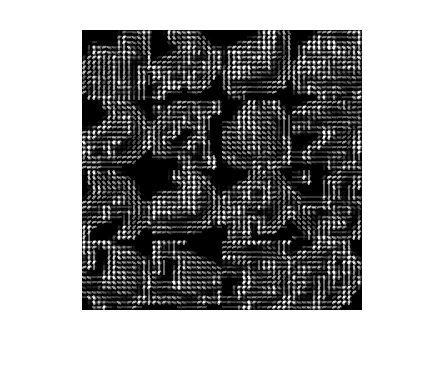
\includegraphics[trim=2mm 15mm 13mm 0mm,
clip,width=0.45\textwidth]{figures/color_hog.png} }
  \subfigure[HOG from depth-mapped images.] {
    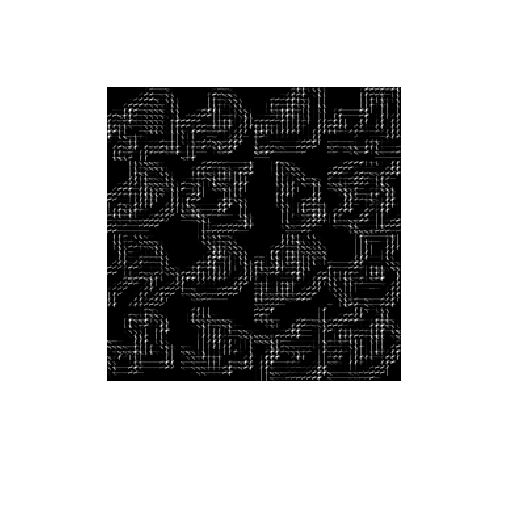
\includegraphics[trim={7mm 35mm 11mm 0cm},
  clip, width=0.5\textwidth]{figures/depth_hog.png}
  }
  \caption{Visualization of HOG descriptors computed from $64\times64$px
  image patches.}
  \label{fig:hand-hog}
\end{figure}

\subsection{Compare HOG from Color or Depth Images}
Using the ChAirGest dataset and the same recognition method, I compared
results using HOG computed from different types of
data. Section~\ref{sec:eval-feature} Table~\ref{tab:comp-feature} shows that
using HOG from both color and depth data gives the highest $F_1$ score. However, the improvement is small
compared with using HOG computed from depth data only. As a result, in the
real-time system, I only use HOG computed from depth data to increase
processing speed.

The reason that HOG from depth data gives better result than HOG from color data
could be that depth data contains more information about the contour the hand in
one more dimension (see Figure~\ref{fig:hand-3d}).
 
\begin{figure}[tbh]
\centering
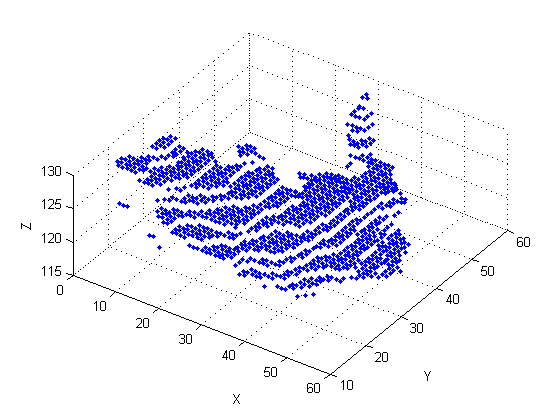
\includegraphics[width=0.5\textwidth]{figures/hand3d.png}
\caption{View of quantized depth data of a hand in 3D.}
\label{fig:hand-3d}
\end{figure}

\section{Principal Component Analysis}
The dimension of the HOG feature descriptor can be large, therefore, I use
Principal Component Analysis (PCA)~\cite{pca} to reduce its dimensionality (see
Appendix~\ref{app:pca} for detail). PCA can be seen as a feature
encoder~\cite{ranzato07}.

The number of principal components is determined through cross-validation. For
the YANG dataset, I use 15 principal components from the HOG feature descriptor.
We use one user's data from the YANG dataset to visualize the PCA
encoded HOG descriptors. Figure~\ref{fig:pca} shows the histograms of the 15
variables after projecting the original HOG descriptors onto the principal
components and then applying standardization.
We observe that the distributions closely follow Gaussian or mixture of
Gaussians distributions.

\begin{figure}[tbh]
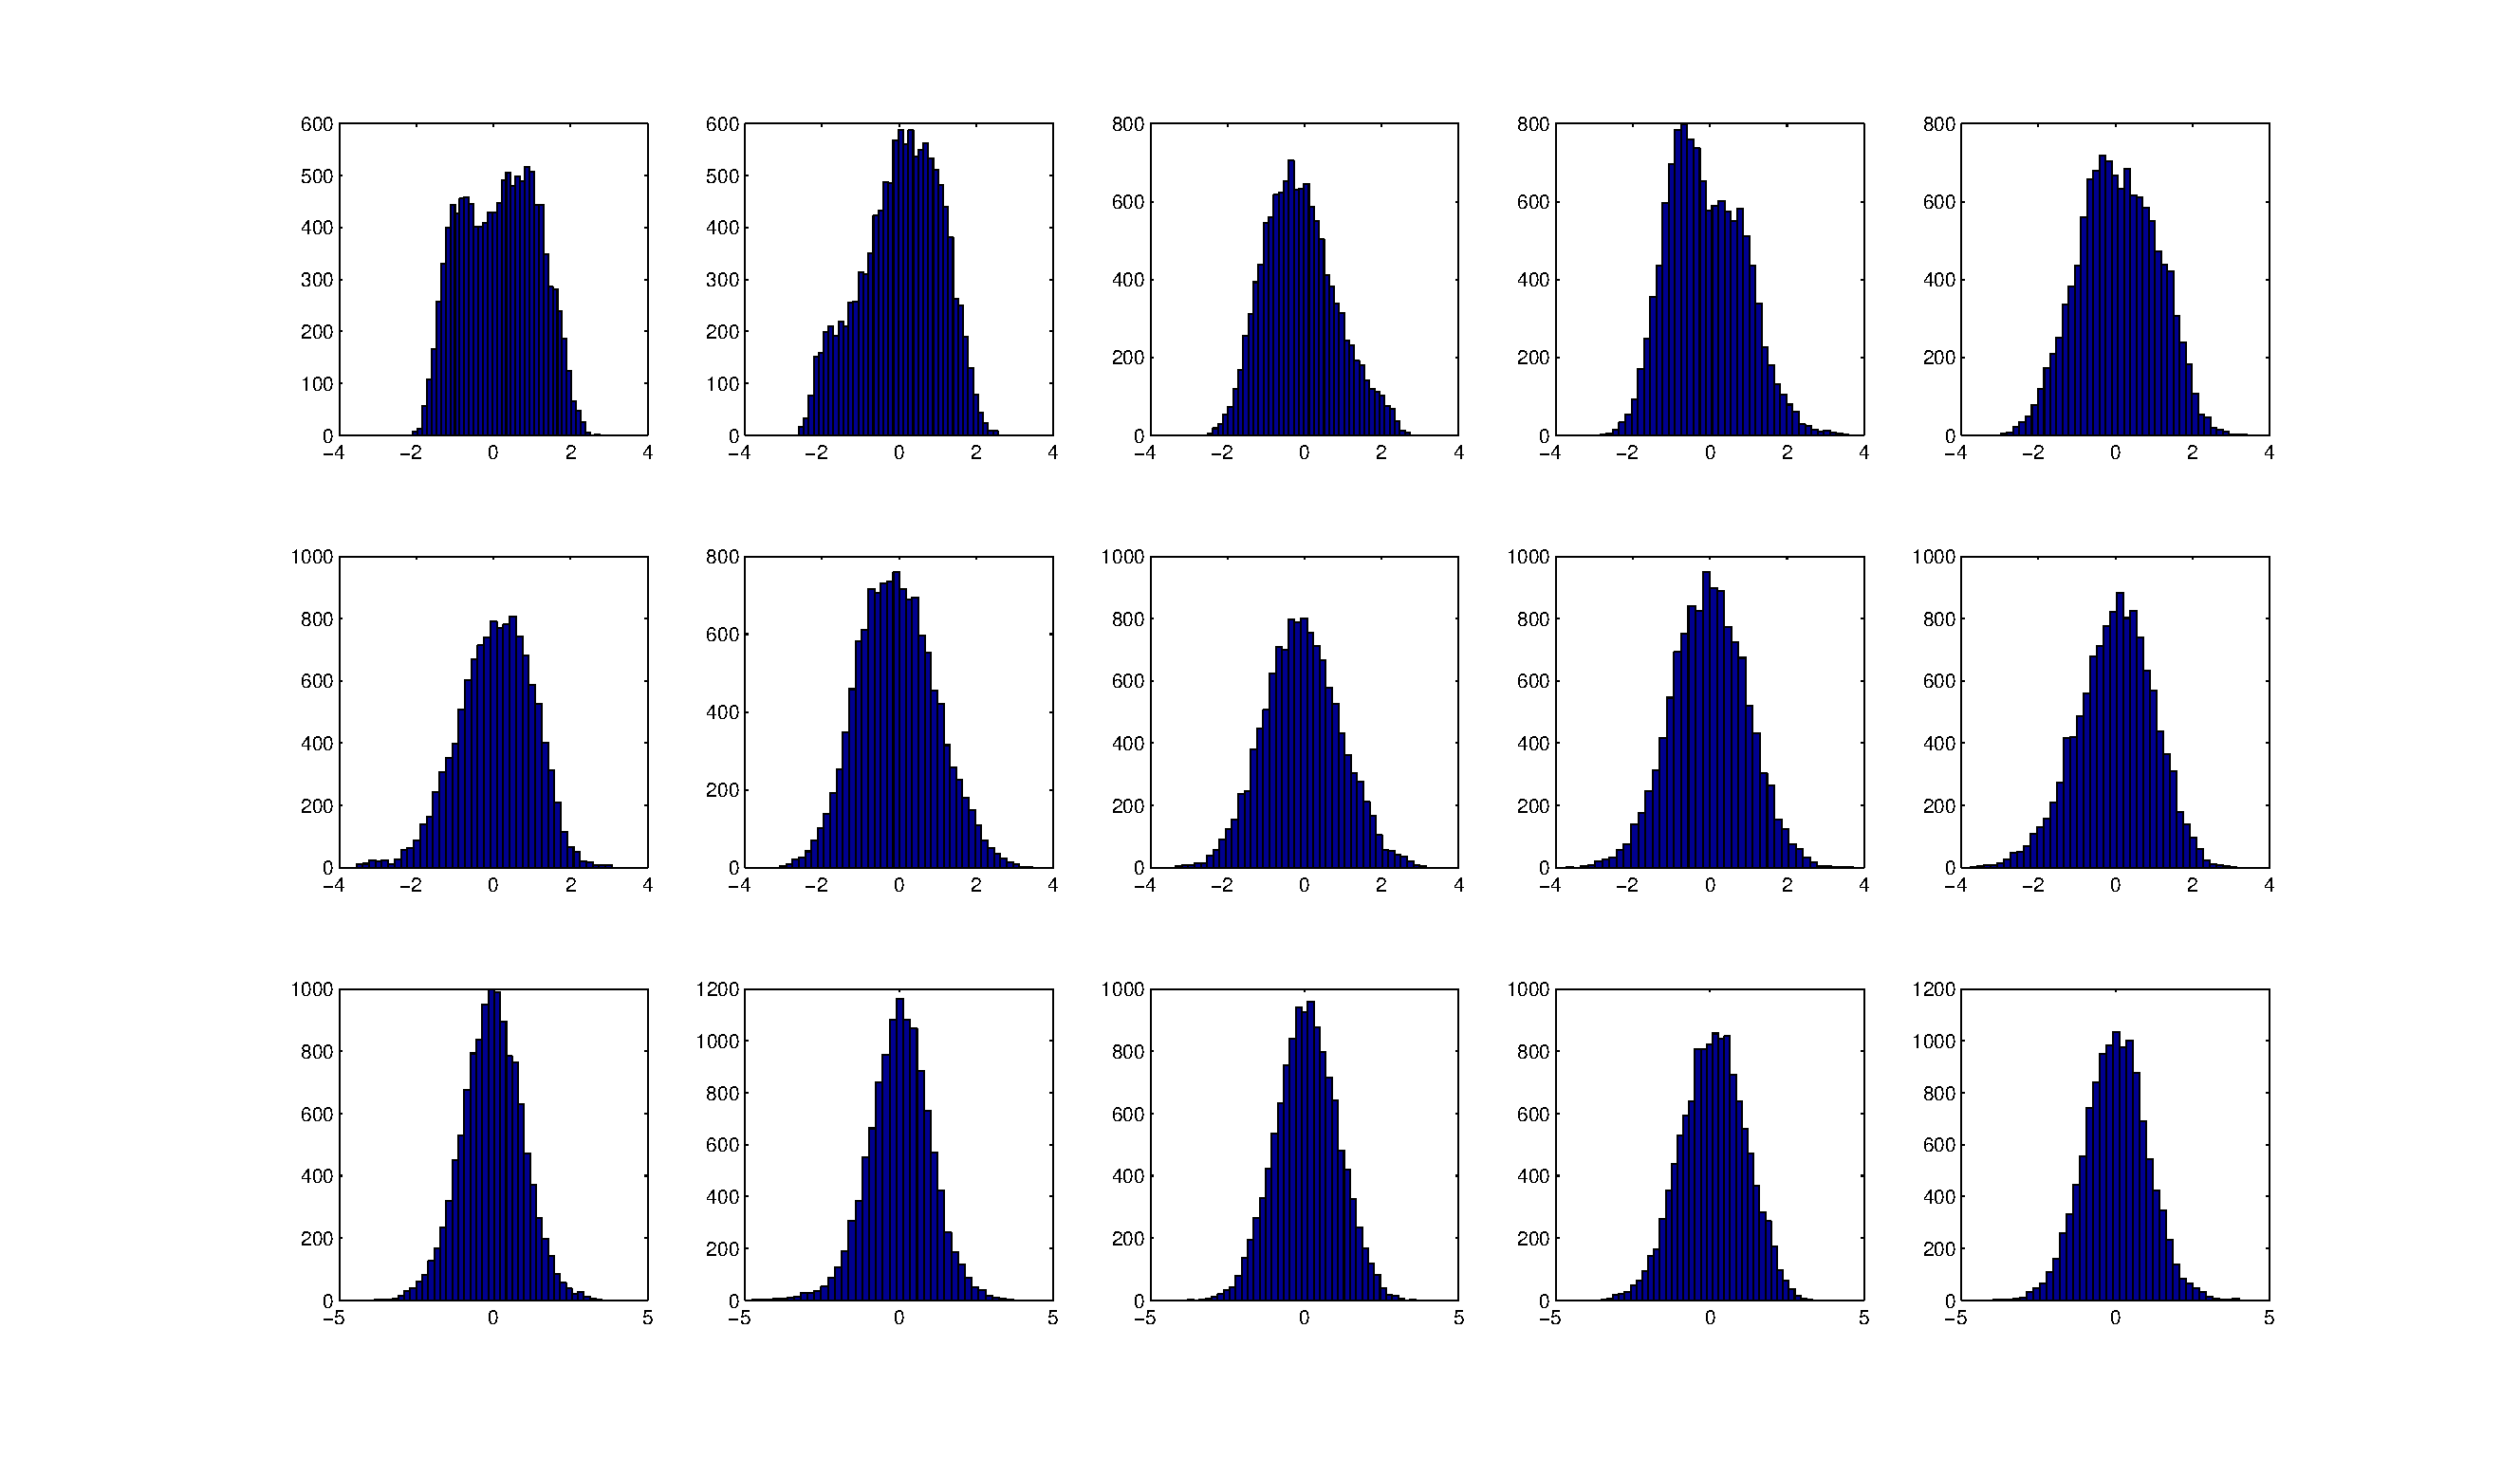
\includegraphics[width=\columnwidth]{figures/hist_pca.eps}
\caption{Histograms of the 15 components of in the feature vectors computed
from apply PCA to the HOG descriptors.}
\label{fig:pca}
\end{figure}

\section{SVM for Encoding Hand Poses}
Similar to Song et al.~\cite{song12}, I attempted to further encode the feature
vectors obtained from PCA into hand pose classes. For each pose
gesture, there is a class for its hand poses, and for all the path
gestures, all of their hand poses are grouped into one class called ``Other''.
Figure~\ref{fig:hand-pose-classes} shows hand pose images from two such classes.

\begin{figure}[tbh]
\centering
\subfigure[Depth-mapped hand pose images from ''POINT'' class.]{
  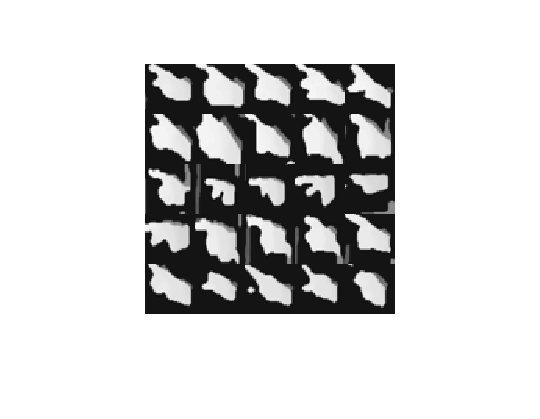
\includegraphics[width=0.5\linewidth,
  trim={0cm 1cm 0cm 0cm}, clip]{figures/point_depth_resize_32_denoise.eps} }
\subfigure[Corresponding HOG descriptor.]{
  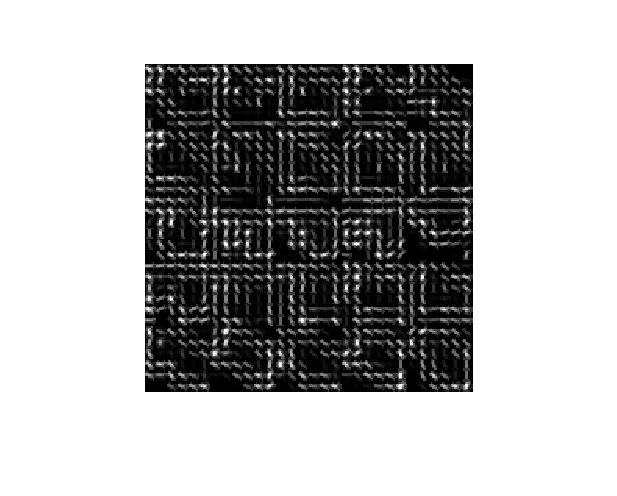
\includegraphics[trim={0cm 1cm 0cm 0cm},
  clip, width=0.45\linewidth]{figures/point_depth_hog.eps} }
\subfigure[Depth-mapped hand pose images from ``OTHER'' class.]{
  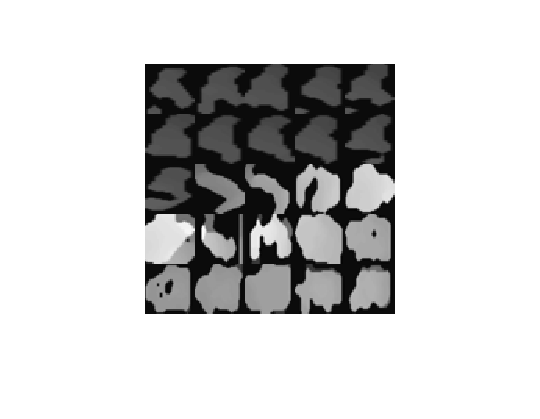
\includegraphics[width=0.5\linewidth,
  trim={0cm 1cm 0cm 0cm}, clip]{figures/other_depth_resize_32_denoise.eps} }
\subfigure[Corresponding HOG descriptor.]{
  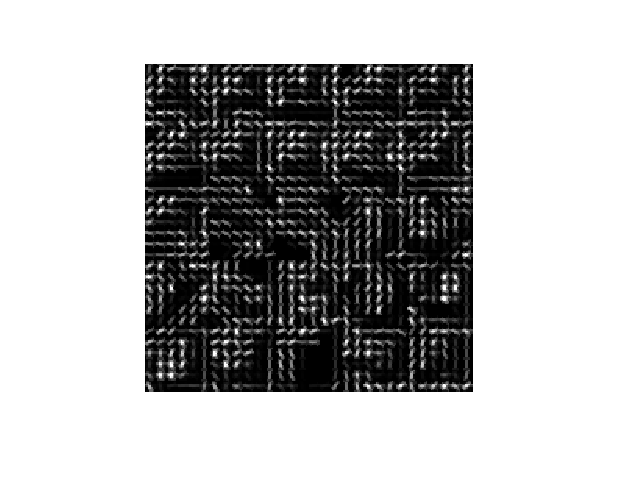
\includegraphics[trim={0cm 1cm 0cm 0cm},
  clip, width=0.45\linewidth]{figures/other_depth_hog.eps} }
\caption{Examples of hand poses from two classes.}
\label{fig:hand-pose-classes}
\end{figure}

I use SVM with
Radial Basis Function (RBF) as the kernel function to do the classification\footnote{
LIBSVM (\url{http://www.csie.ntu.edu.tw/~cjlin/libsvm/}) are used for SVM
related computation.}. Grid search~\cite{hsu10} on the
training data are used to find the misclassification costs and 
$\gamma$ in the RBF kernel function.

It is important to note that the data is highly
unbalanced, for example, there are more instances in the ``Other'' class than
other hand pose classes.
If we ignore the  fact that the data is unbalanced, the resultant classifier
will favor the majority class~\cite{ben2010}. To take this
into account, I assign different misclassification costs, $C_i$, (SVM
soft-margin constants) to each class $i$. If $n_+$ and $n_-$ are the number of
examples in a two -class problem, we choose $C_+$ and $C_-$ such that: 
\begin{align}
\frac{C_+}{C_-} = \frac{n_-}{n_+}
\end{align}
To generalize this to multi-class problems, if $n_1, n_2, \ldots, n_k$ are the
number of examples in a $k$-class problem, we can choose $C_1, C_2, \ldots, C_k$
such as 
\begin{align}
C_1 : C_2 :\ldots : C_k =  \frac{1}{n_1} :  \frac{1}{n_2} : \ldots : 
\frac{1}{n_k}
\end{align}

Using data from one user in the YANG dataset, I compared hand pose
classification results using SVM and my HMM-based gesture recognition algorithm
with mixture of Gaussians (MoG) as the emission probability. There are 5 classes
in total: Point, Palm\_Up, Grab, Rest, and Other. Table~\ref{tab:svm} shows
that using SVM does not give better result.  Figure~\ref{fig:svm-hmm}
shows a visualization of the classification results for a segment in a sequence.
It shows that the HMM-based method has a smoothing effect which helps to improve
performance.

\begin{table}[tbh]
\centering
\begin{tabular}{|l|l|l|l|}
\hline
& \thead{Precision} & \thead{Recall} & \thead{$\mathbf{F_1}$} \\
\hline
SVM & 0.74 & 0.77 & 0.75 \\
\hline
HMM with MoG emission & \textbf{0.81} & \textbf{0.82} & \textbf{0.81} \\
\hline
\end{tabular}
\caption{Comparison of hand pose classification results.}
\label{tab:svm}
\end{table}

\begin{figure}[tbh]
\centering
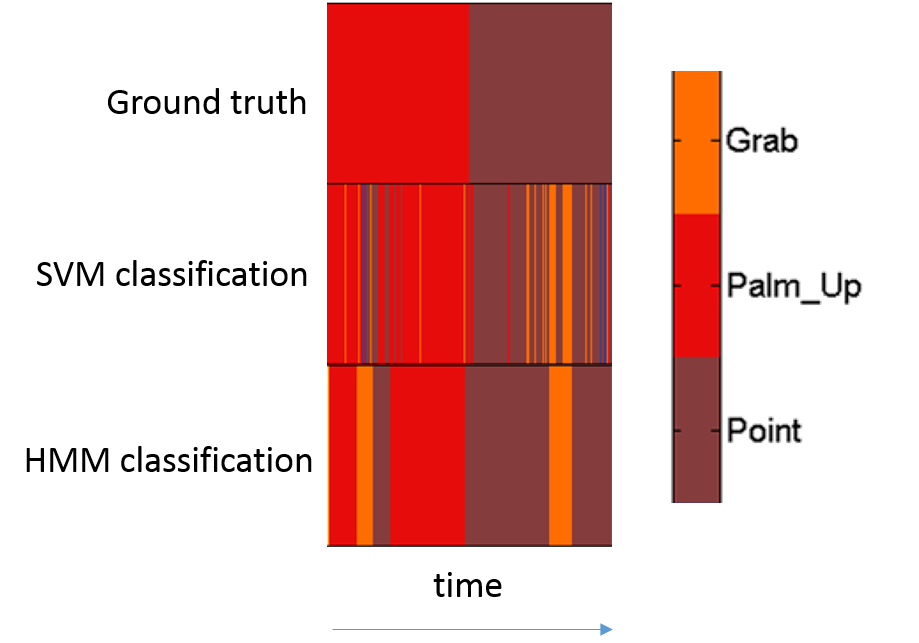
\includegraphics[width=0.5\textwidth]{figures/svm_hmm.png}
\caption{Visualization of the classification results comparing two methods.
this is a continuous segment in a sequence with two pose gestures: ``Palm up''
and ``Point''.}
\label{fig:svm-hmm}
\end{figure}

SVM can output probabilities instead of hard classifications. It is plausible to
use the probabilities as part of the feature vector. However, unlike the other
features in the feature vector, the probabilities for a particular class from
SVM does not follow Gaussian distribution (see Figure~\ref{fig:svm}). 

\begin{figure}[tbh]
\centering
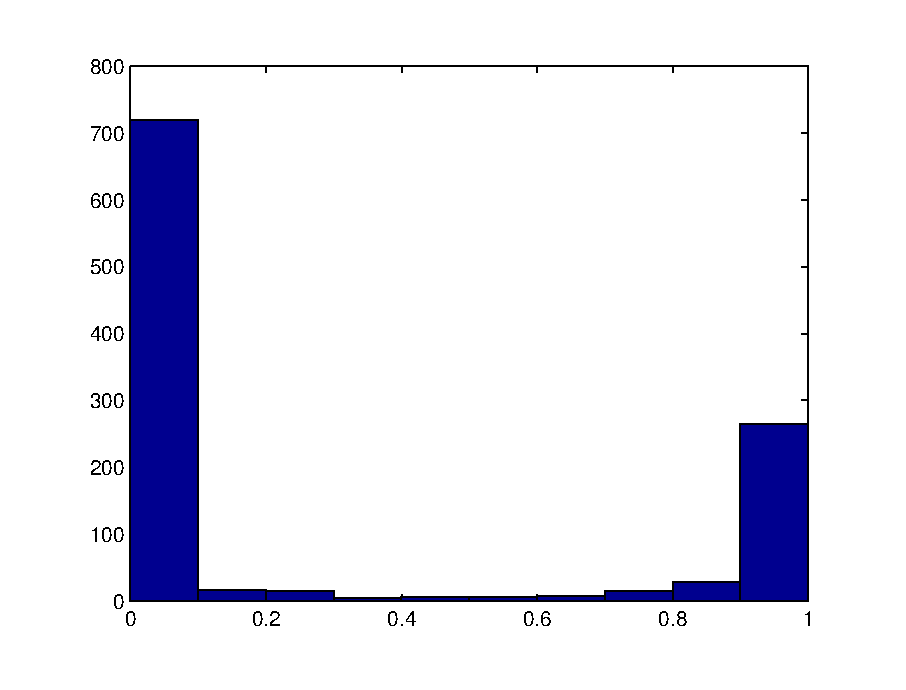
\includegraphics[width=0.55\textwidth]{figures/hist_svm.eps}
\caption{Histogram of SVM probability output for one class.}
\label{fig:svm}
\end{figure}

As a result, it does not seem to be
effective to add SVM encoding (hard decisions or soft decisions) into the
feature vectors.
%\section{Dictionary Learning}

\section{Discussion}
Based on the above analysis, the final feature vector is a concatenation of
motion features and PCA encoded HOG descriptors. All the features follow
Gaussian or MoG distributions, making it is easy to incorporate them in the
HMM-based models.

The probability output from SVM does not follow Gaussian distribution. This
makes it hard to incorporate them into an HMM-base model which models
compatibility between the output and the hidden state using a conditional probability
distribution (CPD). However, probability output might be useful as part of a
feature vector for a CRF-based model as those models have greater flexibility to
incorporate features (e.g. no CPD required). 
